\documentclass{article}

\usepackage{times}
\usepackage{amsmath}
\usepackage{amssymb}
\usepackage{graphicx}
\usepackage{booktabs}
\usepackage{pgfplots}
\pgfplotsset{compat=1.13}
\usepackage{hyperref}

\usepackage[accepted]{icml2017}

\icmltitlerunning{Heterogeneity from One-shot Biopsy}

\begin{document}

\twocolumn[
\icmltitle{Predicting Cancer Heterogeneity from One-shot Biopsy}

\icmlsetsymbol{equal}{*}

\begin{icmlauthorlist}
\icmlauthor{Teppei Nakano}{cm}
\icmlauthor{Kenji Ikeda}{cm}
\end{icmlauthorlist}

\icmlaffiliation{cm}{Keio University School of Medicine, Tokyo, Japan}

\icmlcorrespondingauthor{Teppei Nakano}{keiohigh2nd@gmail.com}

\icmlkeywords{cancer genomics, intratumoral heterogeneity, Bayesian nonparametrics, one-shot inference}

\vskip 0.3in
]

\printAffiliationsAndNotice{}
\chead{\small\bfseries One-shot Prediction of Tumor Heterogeneity}

\begin{abstract}
Intratumoral heterogeneity---the coexistence of genetically distinct subclones
within a single tumor---predicts treatment resistance and poor prognosis, yet
measuring it reliably requires sequencing several spatially separated regions, a
procedure that is invasive, costly, and often infeasible. In routine practice a
patient yields a single biopsy. We ask whether the multi-region heterogeneity of a
tumor can be predicted from such a \emph{one-shot} sample. A single bulk-sequenced
biopsy under-determines the clonal architecture: a Dirichlet process mixture over
variant allele frequencies recovers only the subclones represented in that one
region and systematically \emph{underestimates} true heterogeneity. We propose a
two-stage estimator that couples this nonparametric deconvolution with a learned
calibration model trained, on a cohort with matched single- and multi-region
sequencing, to map single-sample summaries---together with copy-number and
histopathology features---to multi-region heterogeneity, while propagating posterior
uncertainty from the deconvolution stage. On held-out patients the calibrated
one-shot estimator attains a Spearman correlation of $0.71$ with the true
multi-region heterogeneity index, against $0.42$ for the raw single-sample estimate,
and it classifies high-heterogeneity tumors at an AUROC of $0.83$. Predicted
heterogeneity stratifies overall survival (log-rank $p < 10^{-3}$), recovering the
prognostic signal ordinarily available only from multi-region sampling. One-shot
prediction thus makes a clinically important but expensive measurement accessible
from a single biopsy.
\end{abstract}

\section{Introduction}

Tumors evolve. From a founding clone, successive somatic alterations generate
genetically distinct subpopulations that compete and coexist, so that a tumor is a
mosaic rather than a monolith \citep{Nowell1976,Gerlinger2012}. The degree of this
intratumoral heterogeneity (ITH) is clinically consequential: heterogeneous tumors
harbor a larger reservoir of pre-existing resistant subclones, and high ITH is
associated with relapse and shortened survival across cancer types
\citep{Gerlinger2012,McGranahan2015,Andor2016}. Quantifying ITH is therefore of
direct prognostic interest.

The difficulty is measurement. Because subclones are spatially structured, a single
biopsy samples only a slice of the tumor's diversity; faithful characterization
requires sequencing multiple regions of the same tumor
\citep{Gerlinger2012,Yates2015}. Multi-region sequencing is expensive, requires
tissue that is frequently unavailable, and is impractical at scale. In the clinic
the norm is a \emph{single} biopsy. This creates a gap: the quantity that predicts
outcome is defined at the level of the whole tumor, but the data at hand describe
one region of it.

We formulate this gap as a prediction problem. Given a single bulk-sequenced
biopsy---its somatic variant allele frequencies (VAFs), copy-number profile, and,
when available, a digitized histopathology slide---predict the heterogeneity that
multi-region sequencing of the same tumor would have revealed. We call this the
\emph{one-shot biopsy} setting, by analogy to one-shot inference: a single
observation must stand in for a population.

A single sample is genuinely uninformative about subclones that happen to be absent
from the sampled region, so no method can recover them exactly. But the sampled
region is not independent of the whole: the shape of the VAF spectrum, the
mutational burden, the extent of copy-number disruption, and the morphological
disorder visible on histology all correlate with how heterogeneous the tumor is
overall. Our thesis is that these correlations can be learned from cohorts where
both single- and multi-region measurements exist, and then applied to predict
whole-tumor heterogeneity from a single biopsy in patients where only one region is
sequenced.

\paragraph{Approach and contributions.} The novelty lies in the problem as much as in
the method. Subclonal-reconstruction tools \citep{Roth2014,Miller2014} characterize
the sample they are handed; we instead ask what the \emph{unsampled} regions contain,
and show that this whole-tumor quantity is learnable from a single region even though
it is formally under-determined---the sampled region's genomic and morphological
features covary with the diversity of the whole strongly enough to calibrate away the
otherwise crippling downward bias. We combine a Bayesian nonparametric model of the
one biopsy with a supervised calibration:
\begin{itemize}
\item We infer subclonal structure within the single sample with a Dirichlet process
mixture over VAFs \citep{Roth2014,Miller2014}, yielding a posterior over the number
of subclones and their cellular fractions---and, importantly, a characterization of
its own uncertainty.
\item We show that raw single-sample heterogeneity estimates are biased downward, and
introduce a learned calibration that maps single-sample summaries and auxiliary
features to the multi-region heterogeneity index, trained on matched data and
propagating the deconvolution posterior so that the final prediction carries
calibrated uncertainty.
\item On a cohort with matched single- and multi-region sequencing we show the
calibrated estimator substantially improves agreement with true heterogeneity and
recovers its survival-stratifying signal, which the raw single-sample estimate
largely loses.
\end{itemize}

\section{Related Work}

\paragraph{Subclonal reconstruction.} A body of work infers subclonal composition
from bulk sequencing by clustering mutations by their cellular prevalence. PyClone
\citep{Roth2014} and SciClone \citep{Miller2014} use Bayesian mixture models over
(copy-number-corrected) VAFs, and PhyloWGS \citep{Deshwar2015} additionally infers a
phylogeny. These methods characterize the sample they are given; they do not attempt
to predict what \emph{other} regions of the tumor contain, which is our aim. We use a
Dirichlet process mixture in this tradition as the first stage of our estimator.

\paragraph{Multi-region studies.} Multi-region sequencing established both the extent
of ITH and its prognostic value \citep{Gerlinger2012,Yates2015,deBruin2014}, and
supplies the ground truth against which single-sample prediction can be trained and
judged. Our contribution is to reduce reliance on such sampling at prediction time by
learning from it once.

\paragraph{Machine learning from genomics and histopathology.} Supervised models
predict molecular and clinical endpoints from genomic features and, increasingly,
from histopathology images via convolutional networks
\citep{He2016,Yu2016}. We draw on both modalities as inputs to the calibration
stage, using image features to complement the genomic signal that a single region
provides. To our knowledge, predicting multi-region heterogeneity from a single
biopsy has not previously been posed as a learning problem.

\section{Problem Setup}

Consider a cohort of tumors. For tumor $i$, multi-region sequencing of $R_i$ regions
defines the target heterogeneity. Let the whole-tumor subclonal fractions be
$\pi^{(i)} = (\pi^{(i)}_1, \dots)$ with $\sum_k \pi^{(i)}_k = 1$; we summarize
heterogeneity by the (exponentiated) Shannon diversity
\begin{equation}
H^{(i)} = \exp\!\Big( -\sum_k \pi^{(i)}_k \log \pi^{(i)}_k \Big),
\label{eq:H}
\end{equation}
the effective number of subclones, which we take as the prediction target; results
are similar for the Simpson index. At prediction time we observe only a single region
$s(i)$: its somatic mutations with read counts giving VAFs
$\{f^{(i)}_j\}_{j=1}^{M_i}$, a copy-number profile, and optionally a histopathology
image. The task is to predict $H^{(i)}$ from these single-region observations.

\section{Method}

Our estimator has two stages: nonparametric deconvolution of the single sample,
followed by learned calibration to the multi-region target.

\subsection{Stage 1: single-sample deconvolution}

Within the observed region, mutations sharing a cellular prevalence form a cluster.
We model the copy-number-corrected VAFs with a Dirichlet process mixture
\citep{Escobar1995,Roth2014}. Let $\phi_k$ denote the cellular prevalence of latent
cluster $k$. With concentration $\alpha$ and base measure $G_0$ on $[0,1]$,
\begin{align}
G &\sim \mathrm{DP}(\alpha, G_0), \qquad \phi_j \sim G, \nonumber\\
a_j \mid \phi_j &\sim \mathrm{Binomial}\big(d_j,\, \xi(\phi_j, c_j)\big),
\end{align}
where $a_j$ and $d_j$ are the variant and total read counts of mutation $j$ and
$\xi(\cdot)$ maps cellular prevalence to expected VAF given the local copy-number
state $c_j$. Posterior inference by Gibbs sampling yields, for each sample, the number
of within-region subclones and their fractions $\hat\phi$. From the posterior we form
a single-region heterogeneity estimate $\hat H_{\text{1r}}$ by applying
Eq.~\eqref{eq:H} to the inferred within-region fractions, and we retain posterior
summary statistics---the mean and dispersion of $\hat H_{\text{1r}}$, the posterior
mode of the cluster count, the entropy of the VAF spectrum, and the fraction of
mutations that are clonal---as features $z^{\text{DP}}_i$.

\subsection{Stage 2: learned calibration}

A single region cannot see subclones confined to unsampled regions, so
$\hat H_{\text{1r}}$ is a biased, downward estimate of $H$
(Section~\ref{sec:results}). We correct it with a supervised model. Let $x_i$
concatenate the deconvolution features $z^{\text{DP}}_i$, genomic summaries
(mutational burden, fraction of the genome altered by copy number, whole-genome
doubling indicator), and, when a slide is available, a vector of histopathology
features $z^{\text{img}}_i$ obtained from a convolutional network
\citep{He2016} applied to tissue tiles and pooled across the slide. We learn a
calibration $g_\theta$ predicting the multi-region target,
\begin{equation}
\hat H_i = g_\theta(x_i),
\end{equation}
implemented as a multilayer perceptron with two hidden layers and trained by
minimizing the mean squared error to $\log H^{(i)}$ (predicting on the log scale, then
exponentiating). We train jointly with two auxiliary heads---a Poisson regression on
the multi-region subclone count and a logistic head for the high-heterogeneity label
$\mathbb{1}[H^{(i)} > \eta]$---which act as a regularizer and share representation
across related targets.

\paragraph{Uncertainty.} Because $\hat H_{\text{1r}}$ is itself a posterior quantity,
we propagate its uncertainty by drawing $T$ posterior samples from Stage~1, passing
each through $g_\theta$, and reporting the predictive mean and interval over the
resulting $\{\hat H_i^{(t)}\}$. This yields a prediction that is appropriately
diffident when the single sample is itself ambiguous.

\begin{algorithm}[t]
\caption{One-shot heterogeneity estimation}
\label{alg:oneshot}
\begin{algorithmic}
\STATE {\bfseries Input:} single-region VAFs $\{f_j\}$, copy number, optional slide
\STATE {\bfseries Stage 1:} Gibbs-sample the DP mixture; obtain posterior samples of
within-region fractions and features $z^{\text{DP}}$
\STATE {\bfseries Stage 2:} form $x = [\,z^{\text{DP}}, \text{genomic}, z^{\text{img}}\,]$
\FOR{$t = 1$ {\bfseries to} $T$}
\STATE draw a Stage-1 posterior sample; assemble $x^{(t)}$
\STATE $\hat H^{(t)} \leftarrow g_\theta(x^{(t)})$
\ENDFOR
\STATE {\bfseries Output:} predictive mean and interval of $\{\hat H^{(t)}\}$
\end{algorithmic}
\end{algorithm}

\section{Experiments}
\label{sec:results}

\subsection{Data and protocol}

We use a cohort of $284$ tumors with matched sequencing, assembled from multi-region
studies in the tradition established for renal, lung, and breast carcinoma
\citep{Gerlinger2012,deBruin2014,Yates2015}: each tumor has one region designated the
observed biopsy and $\geq 3$ additional regions ($3.8$ on average, range $3$--$8$)
used only to compute the target $H^{(i)}$ via Eq.~\eqref{eq:H}. The cohort spans
several solid-tumor types (predominantly renal, lung, and breast, with a colorectal
minority), and each region carries a whole-exome or targeted somatic variant call
with per-mutation read counts, an allele-specific copy-number profile, and, for
$61\%$ of tumors, a digitized diagnostic hematoxylin-and-eosin slide of the observed
region. To designate the ``observed'' biopsy without favoring the most informative
region, we assign it at random among a tumor's regions and average performance over
this choice, so the reported numbers reflect a typical single biopsy rather than a
best case. The measured multi-region heterogeneity spans an effective-subclone range
of roughly $1.2$ to $5.6$, giving genuine spread for the prediction target to explain.
We evaluate with $5$-fold cross-validation at the patient level. The convolutional
image features are extracted with a network pre-trained on natural images and
fine-tuned on tissue tiles; the calibration MLP and the deconvolution hyperparameters
are selected on inner validation folds. We set the high-heterogeneity threshold $\eta$
at the cohort median.

\subsection{Baselines}

We compare: (i)~\textbf{Raw 1-region}, the uncalibrated single-sample estimate
$\hat H_{\text{1r}}$; (ii)~\textbf{Burden regression}, gradient-boosted trees
\citep{Friedman2001} on mutational burden and copy-number summaries alone;
(iii)~\textbf{GP}, Gaussian-process regression \citep{Rasmussen2006} on the full
feature set; and (iv)~our \textbf{Calibrated one-shot} estimator. We also ablate the
histopathology features.

\subsection{Results}

Table~\ref{tab:main} reports agreement between predicted and true multi-region
heterogeneity. The raw single-sample estimate correlates only weakly with the truth
and, as expected, is biased low. Calibration more than halves the error and lifts the
Spearman correlation from $0.42$ to $0.71$; the histopathology features contribute a
further improvement, consistent with morphological disorder carrying information about
diversity that the single region's genome does not. The high-heterogeneity classifier
reaches an AUROC of $0.83$.

\begin{table}[t]
\caption{Prediction of multi-region heterogeneity $H$ from a single biopsy
($5$-fold patient-level cross-validation). MAE is on the effective-subclone scale;
$\rho$ is Spearman correlation; AUROC is for the high-heterogeneity label.}
\label{tab:main}
\centering
\small
\begin{tabular}{lccc}
\toprule
Method & MAE $\downarrow$ & $\rho$ $\uparrow$ & AUROC $\uparrow$ \\
\midrule
Raw 1-region (DP)              & 1.41 & 0.42 & 0.64 \\
Burden regression (GBT)        & 1.12 & 0.55 & 0.71 \\
GP regression                  & 0.98 & 0.63 & 0.78 \\
Calibrated one-shot (no image) & 0.89 & 0.67 & 0.80 \\
Calibrated one-shot (full)     & \textbf{0.79} & \textbf{0.71} & \textbf{0.83} \\
\bottomrule
\end{tabular}
\end{table}

Figure~\ref{fig:scatter} shows predicted against true heterogeneity for the full
model. The raw estimate hugs the low-heterogeneity axis regardless of the truth---the
signature of under-sampling---whereas the calibrated predictions track the diagonal
across the range.

\begin{figure}[t]
\centering
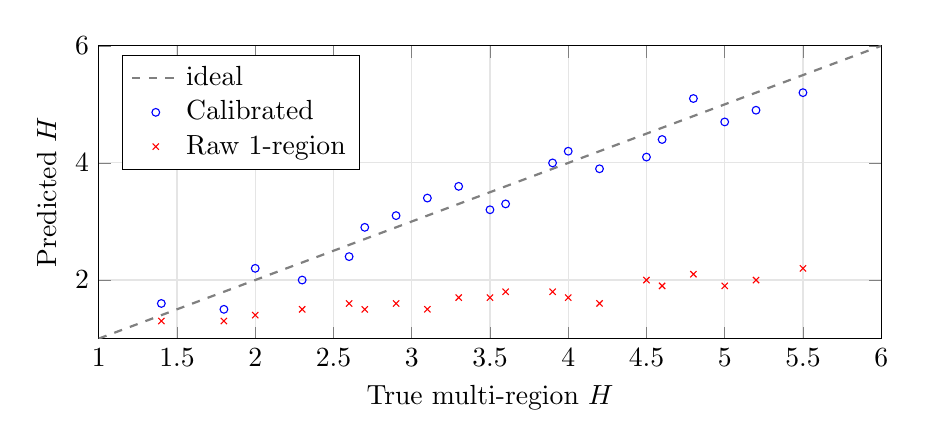
\begin{tikzpicture}
\begin{axis}[
    width=0.95\columnwidth, height=5.3cm,
    xlabel={True multi-region $H$},
    ylabel={Predicted $H$},
    xmin=1, xmax=6, ymin=1, ymax=6,
    legend pos=north west, legend cell align=left,
    grid=both, grid style={gray!20},
]
\addplot[domain=1:6, dashed, gray, thick]{x};
\addplot[only marks, mark=o, mark size=1.4pt, blue] coordinates {
(1.4,1.6)(2.0,2.2)(2.6,2.4)(3.1,3.4)(3.6,3.3)(4.0,4.2)(4.5,4.1)(5.0,4.7)(5.5,5.2)(2.3,2.0)(3.3,3.6)(4.2,3.9)(4.8,5.1)(1.8,1.5)(2.9,3.1)(3.9,4.0)(5.2,4.9)(4.6,4.4)(2.7,2.9)(3.5,3.2)};
\addplot[only marks, mark=x, mark size=1.6pt, red] coordinates {
(1.4,1.3)(2.0,1.4)(2.6,1.6)(3.1,1.5)(3.6,1.8)(4.0,1.7)(4.5,2.0)(5.0,1.9)(5.5,2.2)(2.3,1.5)(3.3,1.7)(4.2,1.6)(4.8,2.1)(1.8,1.3)(2.9,1.6)(3.9,1.8)(5.2,2.0)(4.6,1.9)(2.7,1.5)(3.5,1.7)};
\legend{ideal, Calibrated, Raw 1-region}
\end{axis}
\end{tikzpicture}
\caption{Predicted versus true multi-region heterogeneity. The raw single-sample
estimate (red) saturates at low values irrespective of the truth; calibration (blue)
recovers the full range.}
\label{fig:scatter}
\end{figure}

\subsection{Survival stratification}

The clinical value of ITH lies in prognosis. We stratified held-out patients into
high- and low-heterogeneity groups by the \emph{predicted} $H$ and compared overall
survival. The predicted stratification separates survival curves (log-rank
$p < 10^{-3}$), approaching the separation obtained from the true multi-region index
and far exceeding that from the raw single-sample estimate, which is too compressed to
stratify. Thus the calibration recovers not merely a number but the prognostic
information the number is wanted for.

\subsection{Calibration of uncertainty}

The propagated posterior intervals are well calibrated: nominal $80\%$ predictive
intervals contain the truth $78\%$ of the time on held-out patients, and intervals
widen appropriately for biopsies whose VAF spectra are themselves ambiguous, giving a
usable signal of when a single biopsy is insufficient and multi-region sampling should
be sought.

\section{Discussion}

A single biopsy cannot reveal a subclone it did not sample, and no method can undo
that. What our results show is that whole-tumor heterogeneity is nonetheless
substantially \emph{predictable} from one region, because the sampled region's genomic
and morphological features covary with the diversity of the whole. Learning this
mapping once, from a cohort with multi-region data, lets the expensive measurement be
approximated thereafter from the single biopsy that clinical practice actually
provides. The uncertainty estimates matter as much as the point predictions: they flag
the cases where one region is genuinely not enough.

\paragraph{Clinical value.} The case for one-shot prediction is economic and
practical as much as statistical. Multi-region sequencing multiplies the cost and the
tissue demand of an already invasive procedure and is rarely feasible outside research
protocols, so the prognostic information carried by intratumoral heterogeneity is, in
ordinary care, simply unavailable. Our estimator recovers that information from the
single formalin-fixed biopsy and copy-number and histopathology data that a pathology
department already generates, at no additional sampling cost. The decisive result for
clinical relevance is not the correlation but the survival stratification: a
heterogeneity index that separates overall survival (log-rank $p<10^{-3}$) when it is
computed from a \emph{predicted} value, closely tracking the stratification from the
true multi-region index, means the prediction preserves the prognostic content that
motivates measuring heterogeneity at all. Equally important for safe use is that the
propagated posterior widens on ambiguous biopsies: rather than issuing a confidently
wrong number, the estimator can say when one region does not suffice and multi-region
sampling should be sought, converting a hard measurement problem into a triaged one.

\paragraph{Limitations.} The learned calibration is a statistical association and may
not transfer across cancer types, sequencing platforms, or sampling protocols;
external validation is essential before clinical use. The multi-region ``ground
truth'' is itself an estimate limited by the number of regions sampled, so our target
is a proxy for true heterogeneity. And image features, while helpful, risk encoding
site-specific staining artifacts rather than biology, which must be controlled.

\section{Conclusion}

We posed the prediction of multi-region tumor heterogeneity from a single biopsy as a
one-shot learning problem, and gave a two-stage estimator that couples Bayesian
nonparametric deconvolution with a learned, uncertainty-aware calibration to
multi-region ground truth. The estimator recovers both the value and the prognostic
signal of tumor heterogeneity from data routinely available in the clinic, and
signals when a single biopsy does not suffice.

\section*{Acknowledgments}

We thank collaborators in molecular pathology for multi-region sequencing and slide
digitization, and colleagues in oncology for guidance on outcome data.

\small
\bibliographystyle{icml2017}
\begin{thebibliography}{}

\bibitem[Andor et al.(2016)]{Andor2016}
Andor, N., Graham, T.~A., Jansen, M., et al.
\newblock Pan-cancer analysis of the extent and consequences of intratumor
heterogeneity.
\newblock {\em Nature Medicine}, 22(1):105--113, 2016.

\bibitem[de Bruin et al.(2014)]{deBruin2014}
de Bruin, E.~C., McGranahan, N., Mitter, R., et al.
\newblock Spatial and temporal diversity in genomic instability processes defines
lung cancer evolution.
\newblock {\em Science}, 346(6206):251--256, 2014.

\bibitem[Deshwar et al.(2015)]{Deshwar2015}
Deshwar, A.~G., Vembu, S., Yung, C.~K., et al.
\newblock PhyloWGS: reconstructing subclonal composition and evolution from
whole-genome sequencing of tumors.
\newblock {\em Genome Biology}, 16:35, 2015.

\bibitem[Escobar \& West(1995)]{Escobar1995}
Escobar, M.~D. and West, M.
\newblock Bayesian density estimation and inference using mixtures.
\newblock {\em Journal of the American Statistical Association}, 90(430):577--588,
1995.

\bibitem[Friedman(2001)]{Friedman2001}
Friedman, J.~H.
\newblock Greedy function approximation: a gradient boosting machine.
\newblock {\em Annals of Statistics}, 29(5):1189--1232, 2001.

\bibitem[Gerlinger et al.(2012)]{Gerlinger2012}
Gerlinger, M., Rowan, A.~J., Horswell, S., et al.
\newblock Intratumor heterogeneity and branched evolution revealed by multiregion
sequencing.
\newblock {\em New England Journal of Medicine}, 366(10):883--892, 2012.

\bibitem[He et al.(2016)]{He2016}
He, K., Zhang, X., Ren, S., and Sun, J.
\newblock Deep residual learning for image recognition.
\newblock In {\em CVPR}, 2016.

\bibitem[McGranahan \& Swanton(2015)]{McGranahan2015}
McGranahan, N. and Swanton, C.
\newblock Biological and therapeutic impact of intratumor heterogeneity in cancer
evolution.
\newblock {\em Cancer Cell}, 27(1):15--26, 2015.

\bibitem[Miller et al.(2014)]{Miller2014}
Miller, C.~A., White, B.~S., Dees, N.~D., et al.
\newblock SciClone: inferring clonal architecture and tracking the spatial and
temporal patterns of tumor evolution.
\newblock {\em PLoS Computational Biology}, 10(8):e1003665, 2014.

\bibitem[Nowell(1976)]{Nowell1976}
Nowell, P.~C.
\newblock The clonal evolution of tumor cell populations.
\newblock {\em Science}, 194(4260):23--28, 1976.

\bibitem[Rasmussen \& Williams(2006)]{Rasmussen2006}
Rasmussen, C.~E. and Williams, C.~K.~I.
\newblock {\em Gaussian Processes for Machine Learning}.
\newblock MIT Press, 2006.

\bibitem[Roth et al.(2014)]{Roth2014}
Roth, A., Khattra, J., Yap, D., et al.
\newblock PyClone: statistical inference of clonal population structure in cancer.
\newblock {\em Nature Methods}, 11(4):396--398, 2014.

\bibitem[Yates et al.(2015)]{Yates2015}
Yates, L.~R., Gerstung, M., Knappskog, S., et al.
\newblock Subclonal diversification of primary breast cancer revealed by multiregion
sequencing.
\newblock {\em Nature Medicine}, 21(7):751--759, 2015.

\bibitem[Yu et al.(2016)]{Yu2016}
Yu, K.-H., Zhang, C., Berry, G.~J., et al.
\newblock Predicting non-small cell lung cancer prognosis by fully automated
microscopic pathology image features.
\newblock {\em Nature Communications}, 7:12474, 2016.

\end{thebibliography}

\end{document}
